%----------------------------------------------------------------------------------------
%   PHẦN 3: PHƯƠNG PHÁP TRIỂN KHAI
%----------------------------------------------------------------------------------------
\section{Phương pháp triển khai}

\begin{frame}{Tóm tắt các mô hình sử dụng}
    \begin{table}
        \centering
        \small
        \begin{tabular}{|l|l|l|}
            \hline
            \textbf{Thành phần} & \textbf{Mô hình} & \textbf{Vai trò} \\
            \hline
            Phát hiện xe & YOLOv8n & 5 lớp phương tiện \\
            \hline
            Phát hiện biển số & YOLOv8n & 1 lớp (plate) \\
            \hline
            Mô hình tích hợp & YOLOv8n & 6 lớp (5 xe + plate) \\
            \hline
            Tracking & ByteTrack & Theo dõi đa đối tượng \\
            \hline
            OCR & PaddleOCR + CLAHE & Nhận dạng ký tự biển số \\
            \hline
        \end{tabular}
        \caption{Tổng hợp các mô hình trong hệ thống}
    \end{table}


\end{frame}

%--- SƠ ĐỒ PIPELINE 1 ---
\begin{frame}{Pipeline 1: Sơ đồ triển khai (Two-Stage)}
    \centering
    \begin{tikzpicture}[
        scale=0.95, transform shape,
        node distance=0.5cm and 0.6cm,
        box/.style={rectangle, draw, rounded corners, minimum width=2cm, minimum height=0.7cm, align=center, font=\scriptsize},
        arrow/.style={->, thick, >=stealth}
    ]
        % Row 1
        \node[box, fill=blue!20] (frame) {Frame};
        \node[box, fill=orange!20, right=of frame] (yolo1) {YOLOv8n\\(5 lớp xe)};
        \node[box, fill=yellow!20, right=of yolo1] (track) {ByteTrack};
        \node[box, fill=green!20, right=of track] (crop) {Crop xe};

        % Row 2
        \node[box, fill=red!20, below=1cm of crop] (yolo2) {YOLOv8n\\(plate)};
        \node[box, fill=purple!20, left=of yolo2] (clahe) {CLAHE};
        \node[box, fill=cyan!20, left=of clahe] (ocr) {PaddleOCR};
        \node[box, fill=gray!20, left=of ocr] (valid) {Validation};

        % Arrows Row 1
        \draw[arrow] (frame) -- (yolo1);
        \draw[arrow] (yolo1) -- (track);
        \draw[arrow] (track) -- (crop);

        % Arrow down
        \draw[arrow] (crop) -- (yolo2);

        % Arrows Row 2
        \draw[arrow] (yolo2) -- (clahe);
        \draw[arrow] (clahe) -- (ocr);
        \draw[arrow] (ocr) -- (valid);

        % Labels
        \node[above=0.15cm of yolo1, font=\scriptsize, text=blue] {Detect};
    \end{tikzpicture}

    \vspace{0.3em}
\end{frame}

%--- SƠ ĐỒ PIPELINE 2 ---
\begin{frame}{Pipeline 2: Sơ đồ triển khai (One-Stage)}
    \centering
    \begin{tikzpicture}[
        scale=0.8, transform shape,
        node distance=0.5cm and 0.5cm,
        box/.style={rectangle, draw, rounded corners, minimum width=1.8cm, minimum height=0.7cm, align=center, font=\scriptsize},
        arrow/.style={->, thick, >=stealth}
    ]
        % Row 1: Input and detection
        \node[box, fill=blue!20] (frame) {Frame};
        \node[box, fill=orange!20, right=0.7cm of frame] (yolo) {YOLOv8n\\(6 lớp)};
        \node[box, fill=yellow!20, above right=0.4cm and 0.7cm of yolo] (vehicles) {Vehicles};
        \node[box, fill=green!20, below right=0.4cm and 0.7cm of yolo] (plates) {Plates};
        \node[box, fill=teal!20, right=1.6cm of yolo] (match) {Matching};

        % Row 2: OCR pipeline
        \node[box, fill=purple!20, right=0.6cm of match] (clahe) {CLAHE};
        \node[box, fill=cyan!20, right=of clahe] (ocr) {PaddleOCR};
        \node[box, fill=gray!20, right=of ocr] (valid) {Validation};

        % Arrows
        \draw[arrow] (frame) -- (yolo);
        \draw[arrow] (yolo) -- (vehicles);
        \draw[arrow] (yolo) -- (plates);
        \draw[arrow] (vehicles) -- (match);
        \draw[arrow] (plates) -- (match);
        \draw[arrow] (match) -- (clahe);
        \draw[arrow] (clahe) -- (ocr);
        \draw[arrow] (ocr) -- (valid);

        % Labels
        \node[above=0.15cm of yolo, font=\scriptsize, text=red] {1 inference};
        \node[above=0.15cm of match, font=\scriptsize, text=blue] {plate $\in$ xe?};
    \end{tikzpicture}

    \vspace{0.3em}
\end{frame}

\begin{frame}{Pipeline ALPR chi tiết}
    \begin{block}{Quy trình nhận diện biển số (Pipeline 1)}
    \begin{enumerate}
        \item \textbf{Plate Detection:} YOLOv8n phát hiện vùng biển số
        \item \textbf{Tiền xử lý ảnh:}
        \begin{itemize}
            \item CLAHE (Contrast Limited Adaptive Histogram Equalization)
            \item Grayscale conversion
            \item Noise reduction
        \end{itemize}
        \item \textbf{OCR:} PaddleOCR nhận dạng ký tự
        \item \textbf{Hậu xử lý:}
        \begin{itemize}
            \item Character correction (0$\leftrightarrow$O, 1$\leftrightarrow$I)
            \item Format validation (biển số Việt Nam)
        \end{itemize}
    \end{enumerate}
    \end{block}
\end{frame}

\begin{frame}{Cấu hình huấn luyện}
    \begin{table}
        \centering
        \begin{tabular}{|l|c|c|c|}
            \hline
            \textbf{Tham số} & \textbf{Model 1} & \textbf{Model 2} & \textbf{Tích hợp} \\
            \hline
            Base Model & YOLOv8n & YOLOv8n & YOLOv8n \\
            \hline
            Số lớp & 5 (xe) & 1 (plate) & 6 \\
            \hline
            Image Size & 416×416 & 416×416 & 640×640 \\
            \hline
            Batch Size & 16 & 16 & 64 \\
            \hline
            Epochs & 100 & 100 & 100 \\
            \hline
            Optimizer & SGD & AdamW & SGD \\
            \hline
        \end{tabular}
        \caption{Cấu hình huấn luyện 3 mô hình}
    \end{table}
\end{frame}

\begin{frame}{Dữ liệu huấn luyện}
    \begin{columns}
        \column{0.5\textwidth}
        \textbf{Dataset phát hiện xe:}
        \begin{itemize}
            \item Nguồn: CCTV + Camera thực tế
            \item Quy mô: >16,000 ảnh
            \item Labels: >65,000 boxes
            \item 5 lớp: ô tô, xe máy, xe buýt, xe tải, xe đạp
        \end{itemize}

        \column{0.5\textwidth}
        \textbf{Dataset biển số (VNLP):}
        \begin{itemize}
            \item Nguồn: Thu thập thực tế
            \item Đa dạng: Nhiều góc độ, ánh sáng
            \item Biển số Việt Nam: 1 hàng, 2 hàng
            \item Fine-tuned từ pretrained weights
        \end{itemize}
    \end{columns}

    \vspace{1em}
    \begin{figure}
        \centering
        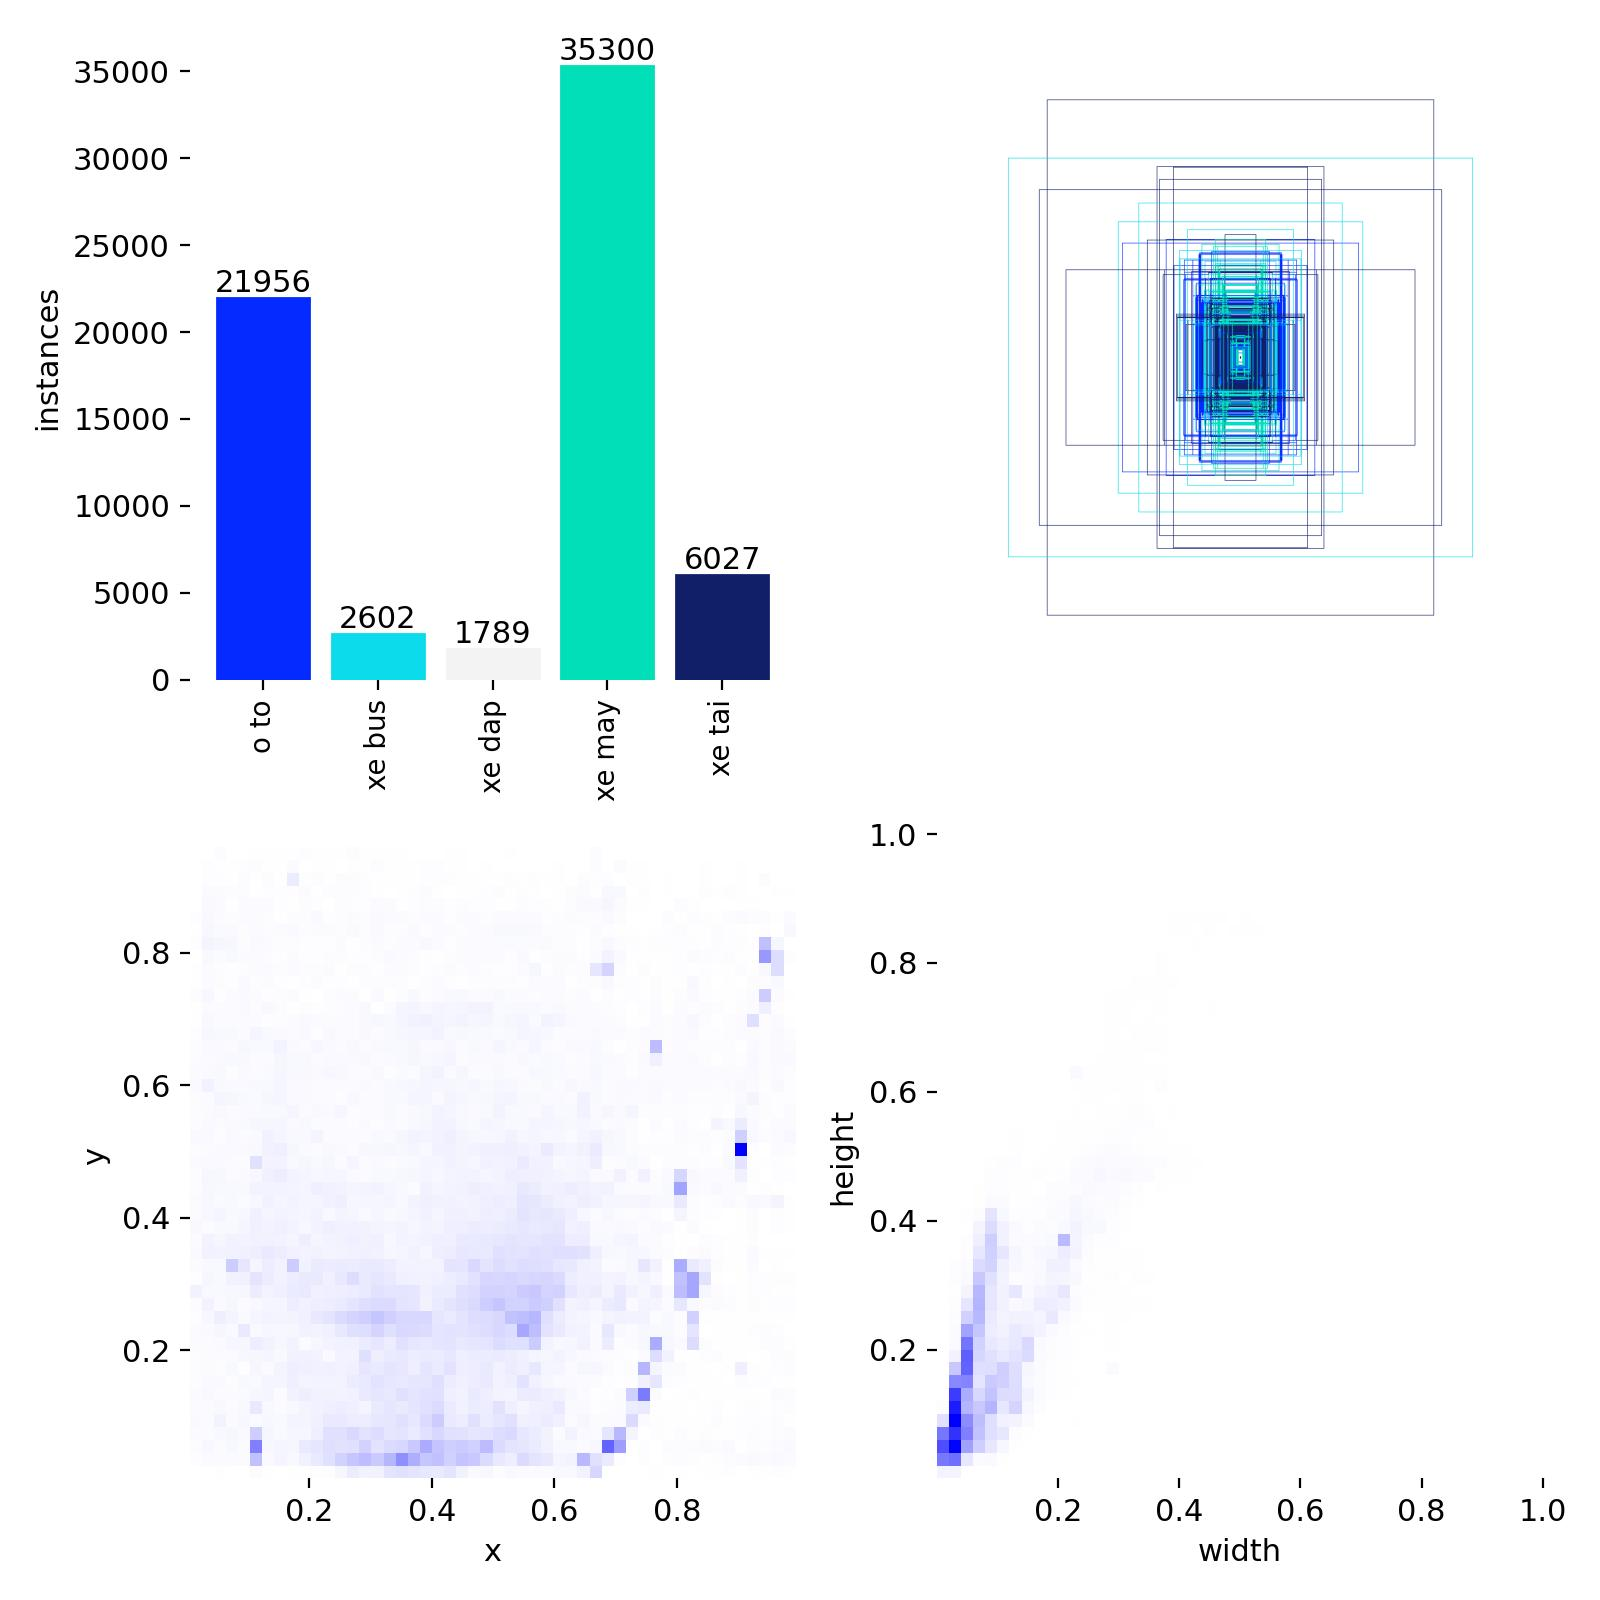
\includegraphics[width=0.5\linewidth]{Figures/labels.jpg}
        \caption{Phân bố nhãn trong dataset phương tiện}
    \end{figure}
\end{frame}

%--- PIPELINE 2 CHI TIẾT ---
\begin{frame}{Pipeline 2: Mô hình tích hợp 6 lớp}
    \begin{block}{Ý tưởng: Huấn luyện 1 model phát hiện đồng thời xe và biển số}
    \begin{enumerate}
        \item Frame $\rightarrow$ YOLOv8n (6 lớp) $\rightarrow$ \{Vehicles, Plates\}
        \item \textbf{Matching:} Kiểm tra Plate nằm trong Vehicle (Containment)
        \item Crop biển số $\rightarrow$ CLAHE $\rightarrow$ PaddleOCR
        \item Format Validation + Retry
    \end{enumerate}
    \end{block}

    \textbf{Ưu điểm so với Pipeline 1:}
    \begin{itemize}
        \item Chỉ 1 lần forward pass qua YOLO (nhanh hơn 2--3x)
        \item Mapping plate$\rightarrow$xe tự động qua containment check
        \item Tiết kiệm GPU Memory (~1.2GB vs ~2.5GB)
        \item Model học được mối quan hệ không gian xe--biển số
    \end{itemize}
\end{frame}

%--- TẠO DỮ LIỆU PIPELINE 2 ---
\begin{frame}{Tạo dữ liệu cho Pipeline 2: Vấn đề}
    \begin{alertblock}{Vấn đề}
    \begin{itemize}
        \item Dataset phương tiện (vietnam\_vehicle\_dataset): \textbf{chỉ có 5 lớp xe}
        \item Dataset biển số (VNLP): \textbf{chỉ có 1 lớp plate}
        \item \textbf{Cần:} Dataset 6 lớp (5 xe + plate) để huấn luyện model tích hợp
    \end{itemize}
    \end{alertblock}

    \begin{block}{Giải pháp: Semi-supervised Labeling}
    Sử dụng Model 2 (đã train trên VNLP, mAP 99.5\%) làm \textbf{Teacher Model} để tự động gán nhãn biển số cho dataset xe
    \end{block}
\end{frame}

\begin{frame}{Tạo dữ liệu Pipeline 2: Quy trình chi tiết}
    \centering
    \begin{tikzpicture}[
        scale=0.8, transform shape,
        node distance=0.3cm and 0.5cm,
        box/.style={rectangle, draw, rounded corners, minimum width=2cm, minimum height=0.6cm, align=center, font=\tiny},
        arrow/.style={->, thick, >=stealth}
    ]
        % Row 1
        \node[box, fill=blue!20] (dataset) {Dataset xe\\(5 lớp)};
        \node[box, fill=orange!20, right=of dataset] (teacher) {Teacher Model\\(mAP 99.5\%)};
        \node[box, fill=green!20, right=of teacher] (infer) {Inference\\toàn bộ ảnh};
        \node[box, fill=yellow!20, right=of infer] (detect) {Phát hiện\\bbox plate};
        \node[box, fill=purple!20, right=of detect] (merge) {Merge\\annotation};
        \node[box, fill=cyan!20, right=of merge] (result) {Dataset\\6 lớp};

        % Arrows
        \draw[arrow] (dataset) -- (teacher);
        \draw[arrow] (teacher) -- (infer);
        \draw[arrow] (infer) -- (detect);
        \draw[arrow] (detect) -- (merge);
        \draw[arrow] (merge) -- (result);
    \end{tikzpicture}

    \vspace{0.5em}
    \begin{block}{Các bước chi tiết}
    \begin{enumerate}
        \item \textbf{Chuẩn bị:} Dataset xe (16,000+ ảnh, 5 lớp) + Teacher Model (YOLOv8n)
        \item \textbf{Inference:} Chạy Teacher trên từng ảnh $\rightarrow$ Phát hiện bbox biển số
        \item \textbf{Lọc:} Chỉ giữ bbox có confidence > 0.5
        \item \textbf{Merge:} Thêm bbox plate (class\_id = 5) vào file annotation gốc
        \item \textbf{Kết quả:} Dataset 6 lớp (5 xe + 1 plate) sẵn sàng huấn luyện
    \end{enumerate}
    \end{block}
\end{frame}

\begin{frame}{Tạo dữ liệu Pipeline 2}


    \begin{alertblock}{Lưu ý}
    \begin{itemize}
        \item Chỉ thêm bbox có confidence > 0.5
        \item Không xóa nhãn xe gốc (5 lớp)
        \item Kết quả: ~65,000 boxes xe + ~X boxes plate
    \end{itemize}
    \end{alertblock}
\end{frame}

\begin{frame}{Pipeline 2: Trade-off sau khi huấn luyện}
    \begin{table}
        \centering
        \small
        \begin{tabular}{|l|c|c|}
            \hline
            \textbf{Metric} & \textbf{Model 2 (VNLP)} & \textbf{Model tích hợp} \\
            \hline
            Số lớp & 1 (plate) & 6 (5 xe + plate) \\
            \hline
            mAP@50 (plate) & \textbf{99.5\%} & 59\% \\
            \hline
            Tốc độ (FPS) & -- & 15--20 FPS \\
            \hline
            GPU Memory & ~0.8GB & ~1.2GB \\
            \hline
        \end{tabular}
    \end{table}

    \textbf{Nguyên nhân mAP plate giảm:}
    \begin{itemize}
        \item \textbf{Class imbalance:} Số lượng xe >> số lượng biển số
        \item \textbf{Kích thước nhỏ:} Biển số chiếm diện tích rất nhỏ trong ảnh
        \item \textbf{Annotation noise:} Gán nhãn tự động có thể bỏ sót biển mờ/nhỏ
    \end{itemize}
\end{frame}

\begin{frame}{Pipeline 2: Gán nhãn bán giám sát (Semi-supervised)}
    \textbf{Vấn đề:} Dataset xe (5 lớp) không có nhãn biển số

    \begin{block}{Quy trình gán nhãn tự động}
    \begin{enumerate}
        \item \textbf{Teacher Model:} Dùng Model 2 (mAP 99.5\%) đã huấn luyện
        \item \textbf{Inference:} Chạy Teacher trên toàn bộ ảnh dataset xe
        \item \textbf{Merge:} Thêm bbox biển số vào annotation gốc
        \item \textbf{Kết quả:} Dataset 6 lớp (5 xe + 1 plate)
    \end{enumerate}
    \end{block}

    \begin{alertblock}{Trade-off}
    mAP plate giảm từ 99.5\% xuống 59\% do:
    \begin{itemize}
        \item Class imbalance (biển số ít hơn nhiều so với xe)
        \item Kích thước biển số nhỏ trong image size 416px
    \end{itemize}
    \end{alertblock}
\end{frame}

%--- TIỀN XỬ LÝ OCR ---
\begin{frame}{Tiền xử lý ảnh biển số}
    \begin{columns}
        \column{0.5\textwidth}
        \textbf{Bước 1: CLAHE}
        \begin{itemize}
            \item Cải thiện độ tương phản
            \item clipLimit = 2.0
            \item tileGridSize = (8, 8)
            \item Hiệu quả với ảnh tối/sáng không đều
        \end{itemize}

        \column{0.5\textwidth}
        \textbf{Bước 2: Sharpening}
        $$ K = \begin{bmatrix} 0 & -1 & 0 \\ -1 & 5 & -1 \\ 0 & -1 & 0 \end{bmatrix} $$
        Làm sắc nét cạnh ký tự
    \end{columns}

    \vspace{0.5em}
    \begin{block}{Character Correction}
    Hiệu chỉnh theo vị trí trong biển số:
    \begin{itemize}
        \item Vị trí 0-1: Chữ số (mã tỉnh) $\rightarrow$ O $\rightarrow$ 0
        \item Vị trí 2: Chữ cái (seri) $\rightarrow$ 0 $\rightarrow$ O
        \item Vị trí 3+: Chữ số $\rightarrow$ B $\rightarrow$ 8
    \end{itemize}
    \end{block}
\end{frame}

%--- FORMAT VALIDATION ---
\begin{frame}{Validation biển số Việt Nam}
    \begin{block}{Định dạng biển số hợp lệ}
    \begin{itemize}
        \item \textbf{Xe máy:} xxYZxxxxx (8-9 ký tự)
        \begin{itemize}
            \item xx: Mã tỉnh (2 số)
            \item Y: Seri (1 chữ)
            \item Z: Số/chữ
            \item xxxxx: 4-5 số cuối
            \item VD: \texttt{29B12345}, \texttt{30M04019}
        \end{itemize}
        \item \textbf{Ô tô:} xxYxxxxx (7-8 ký tự)
        \begin{itemize}
            \item VD: \texttt{51A1234}, \texttt{30H12345}
        \end{itemize}
    \end{itemize}
    \end{block}

    \textbf{Retry Mechanism:}
    \begin{itemize}
        \item Chỉ lưu kết quả đúng format (validated)
        \item Sai format $\rightarrow$ retry frame tiếp theo
        \item Đã có kết quả valid $\rightarrow$ dừng OCR cho xe đó
    \end{itemize}
\end{frame}
